\chapter{Progettazione concettuale}
    \section{Class Diagram}
    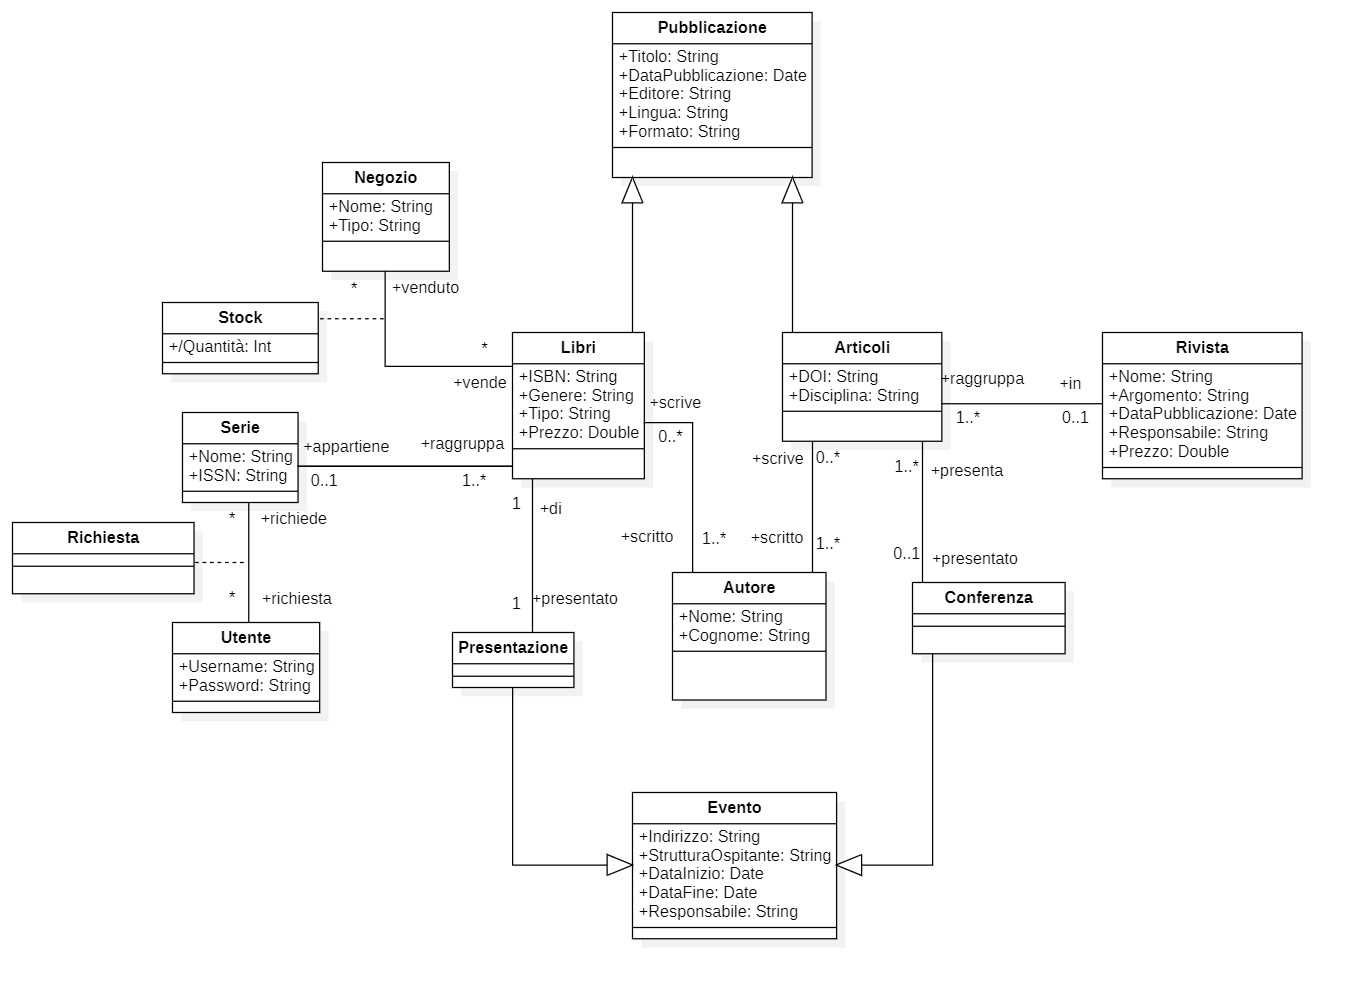
\includegraphics[scale=0.15]{Immagini/SchemaConcettuale.png}
    \section{Analisi della ristrutturazione del Class Diagram}
    Durante questa fase, verranno apportate alcune modifiche al diagramma delle 
    classi al fine di renderlo pi\`u adatto per una traduzione al modello logico.
        \subsection{Analisi delle ridondanze}
        L`unica ridondanza presente nel diagramma \`e l'attributo \textit{DataPubblicazione} nella 
        classe \textbf{Rivista}. Dato che un articolo scientifico deve essere pubblicato in una rivista oppure in una conferenza,
        abbiamo deciso di rimuovere l'attributo dalla classe \textbf{Rivista} e conservare solo quello della classe 
        \textbf{Articolo}, che pu\`o essere comunque accessibile tramite una JOIN.
        \subsection{Analisi degli identificativi}
        In questa fase andremo a scegliere un attributo per identificare univocamente
        le varie entit\`a presenti nello schema precedente, in particolare:
            \begin{enumerate}
            \item L'entit\`a \textbf{Libro} presenta l'attributo \textit{ISBN} che rappresenta una possibile chiave primaria,
                  tuttavia \`e stato scelto di aggiungere un attributo \textit{ID\_Libro} in modo tale da aumentare
                  la velocit\`a di accesso agli indici e garantire l'immutabilit\`a della base di dati.
            \item Per \textbf{Articolo scientifico} la situazione \`e analoga, \`e stato quindi aggiunto un attributo
                  \textit{ID\_Articolo}.
            \item Nel caso dell'entit\`a \textbf{Rivista}, la quale presenta un attributo ISSN che \`e chiave candidata,
                  è stato scelto di inserire un ulteriore attributo \textit{ID\_Rivista}.
            \item Sarebbe possibile identificare un \textbf{Evento} tramite un insieme piuttosto ampio di attributi, \`e
                  stato quindi aggiunto un attributo \textit{ID\_Evento}.
            \item Per lo stesso motivo di Evento, \`e stato aggiunto alla tabella \textbf{Autore} un attributo \textit{ID\_Autore}.
            \item Dato che l'entit\`a \textbf{Negozio} non presenta alcuna chiave candidata, \`e stato aggiunto l'attributo
                  \textit{ID\_Negozio}.
            \item \`E stato deciso di aggiungere a \textbf{Serie} un attributo \textit{ID\_Serie} per ridurre il volume degli
                  indici associati.
            \end{enumerate}
        \subsection{Rimozione degli attributi multivalore}
            Non sono presenti attributi multivalore.
        \subsection{Rimozione degli attributi composti}
            Non sono presenti attributi composti.
        \subsection{Partizione/Accorpamento delle associazioni}
        L`unica associazione 1:1 presente in questo Class Diagram \`e quella tra un \textbf{Libro} e una \textbf{Presentazione},
        nonostante ci\`o, \`e stato deciso di mantenere la classe associativa tra le classi perch\'e abbiamo ritenuto pi\`u idoneo
        avere due classi diverse per associare due tipi di pubblicazione diversi a un Evento.

            
        \subsection{Rimozione delle gerarchie}
            In questo diagramma sono presenti 2 generalizzazioni e 4 relative specializzazioni.
            In particolare:

            Per quanto riguarda la generalizzazione \textbf{Pubblicazione}, si \`e scelto di accorpare l'entit\`a padre
            nelle entit\`a figlie, ottenendo come risultato:
            \begin{itemize}
                  \item Una entit\`a \textbf{Libro} aventi tutti gli attributi di \textbf{Pubblicazione} pi\`u
                        gli attributi della precedente entit\`a \textbf{Libro}.
                  \item Analogamente, l'entit\`a \textbf{Articolo} avr\`a come attributi, quelli di \textbf{Pubblicazione}
                        uniti agli attributi di \textbf{Articolo}.
            \end{itemize}
    
    \section{Class Diagram ristrutturato}
    \subsection{UML Diagram}
    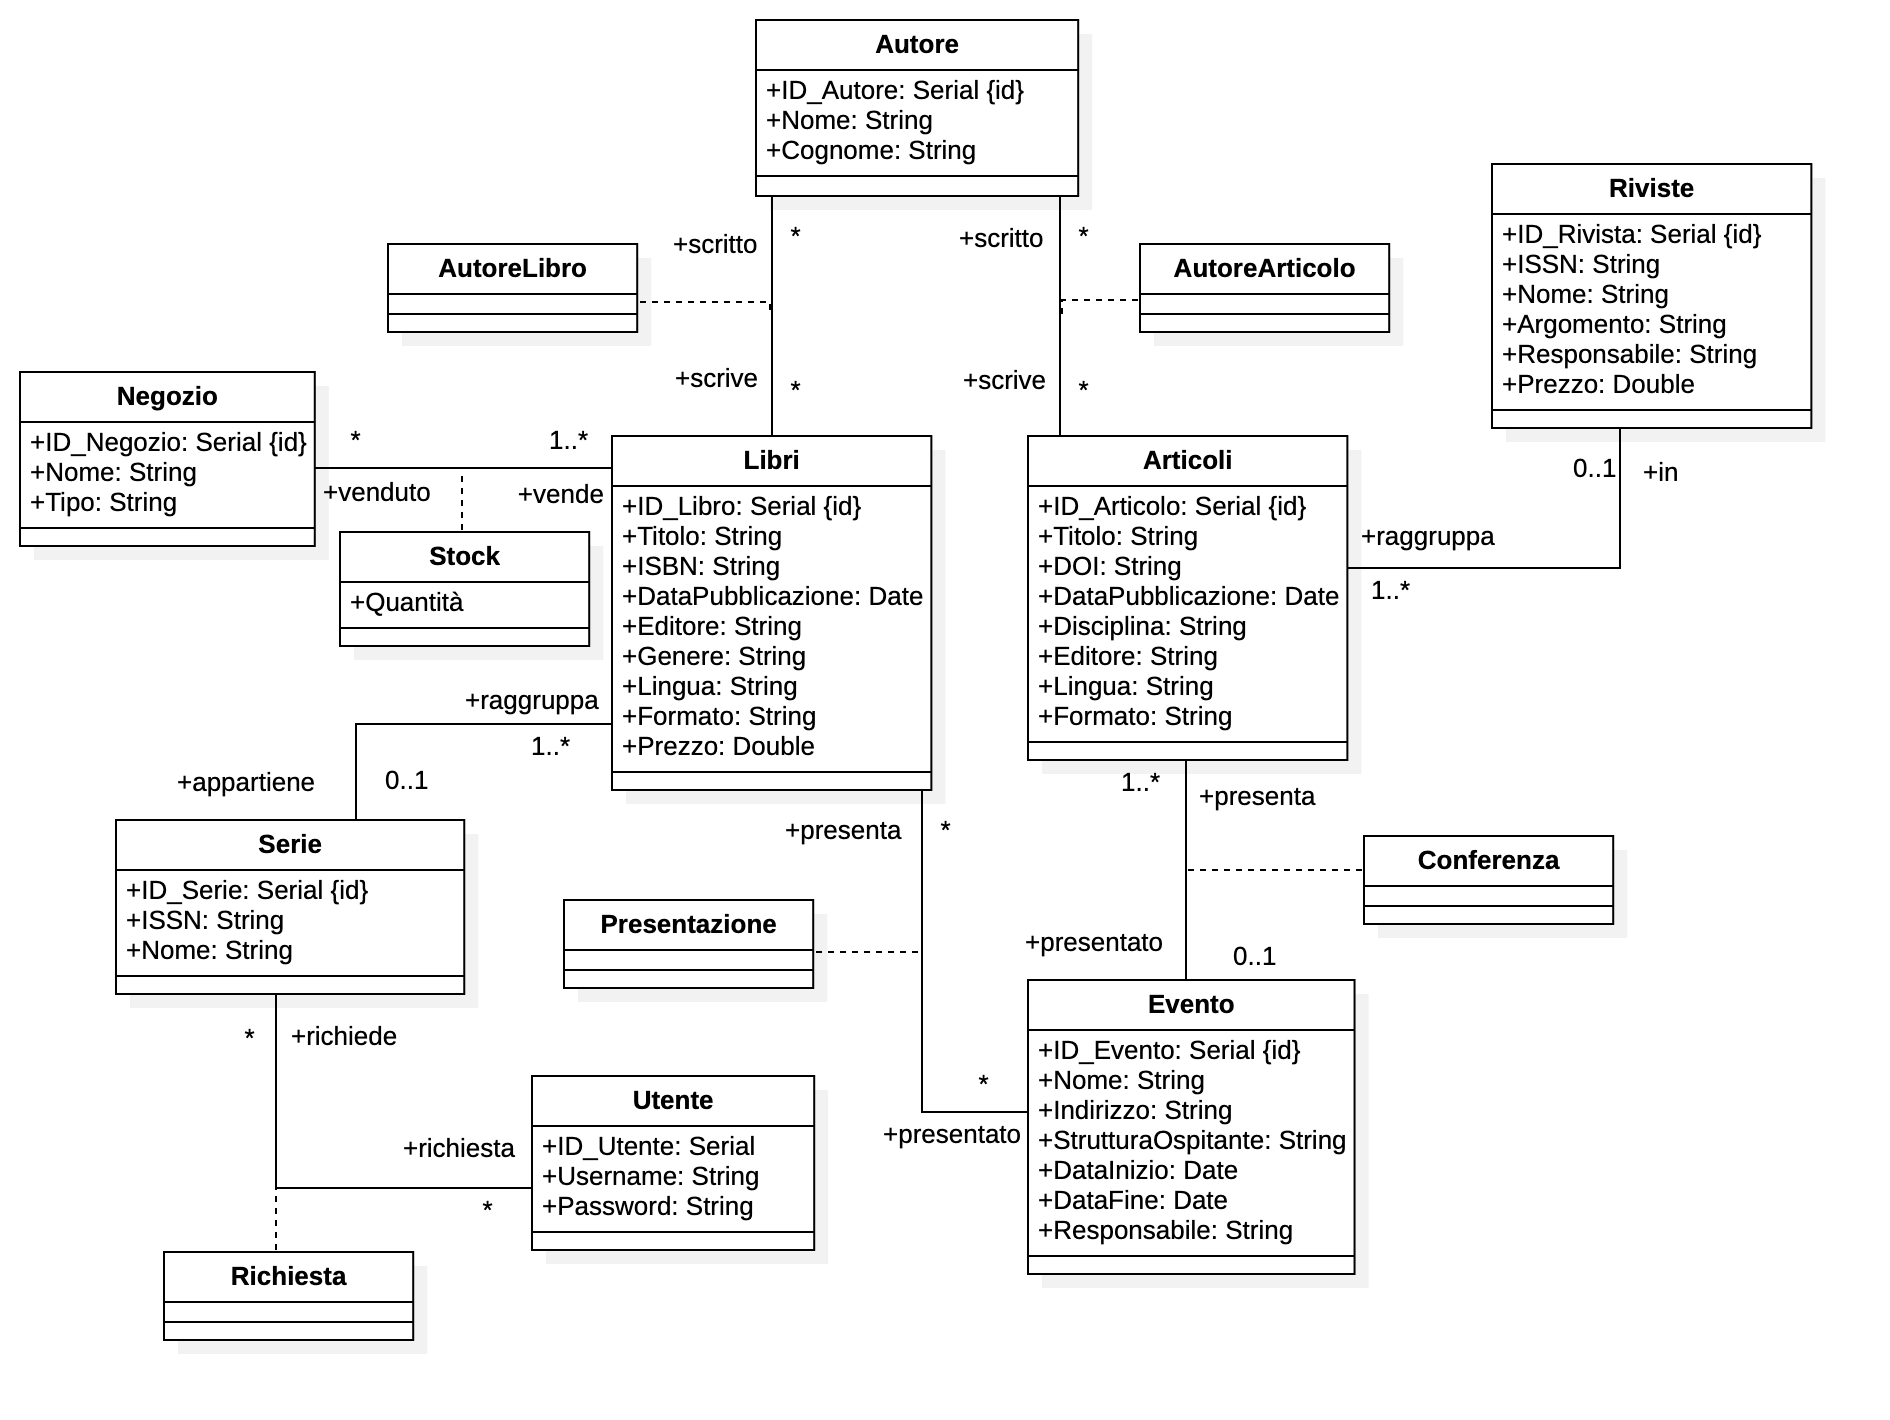
\includegraphics[scale=0.18]{Immagini/SchemaRistrutturato.png}
    \subsection{ER Diagram}
    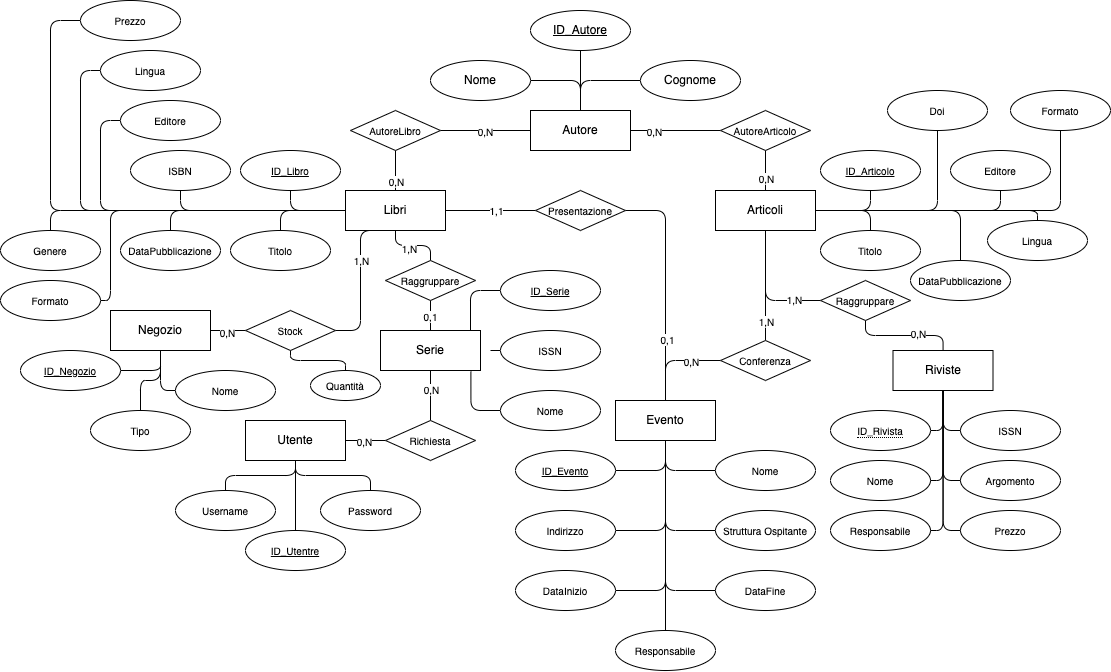
\includegraphics[scale=0.30]{Immagini/ER.png}
    \section{Dizionario delle classi}
    \begin{longtable}{lll}
      \hline
      \multicolumn{1}{|l|}{Classe}           & \multicolumn{1}{l|}{Attributi}                                                                                                                            & \multicolumn{1}{l|}{Descrizione}                                                                                                                                                              \\ \hline
      \endhead
      %
      \multicolumn{1}{|l|}{Articolo}         & \multicolumn{1}{l|}{\begin{tabular}[c]{@{}l@{}}ID\_Articolo\\ Titolo\\ Doi\\ DataPubblicazione\\ Disciplina \\ Editore\\ Lingua\\ Formato\end{tabular}}                 & \multicolumn{1}{l|}{\begin{tabular}[c]{@{}l@{}}Classe che conserva le \\ informazioni relative\\ agli articoli presenti\\ nel sistema\end{tabular}}                                           \\ \hline
      \multicolumn{1}{|l|}{Autore}           & \multicolumn{1}{l|}{\begin{tabular}[c]{@{}l@{}}ID\_Autore\\ Nome\\ Cognome\end{tabular}}                                                                  & \multicolumn{1}{l|}{\begin{tabular}[c]{@{}l@{}}Classe che conserva le\\ informazioni relative\\ agli autori presenti\\ nel sistema\end{tabular}}                                              \\ \hline
      \multicolumn{1}{|l|}{Rivista}          & \multicolumn{1}{l|}{\begin{tabular}[c]{@{}l@{}}ID\_Rivista\\ ISSN\\ Nome\\ Argomento \\ Responsabile \\ Prezzo\end{tabular}}                     & \multicolumn{1}{l|}{\begin{tabular}[c]{@{}l@{}}Classe che conserva le\\ informazioni relative\\ alle riviste scientifiche\\ presenti nel sistema\end{tabular}}                                \\ \hline
      \multicolumn{1}{|l|}{AutoreArticolo}   & \multicolumn{1}{l|}{\begin{tabular}[c]{@{}l@{}}\end{tabular}}                                                                            & \multicolumn{1}{l|}{\begin{tabular}[c]{@{}l@{}}Classe che conserva\\ le informazioni sugli\\ autori degli articoli\\ scientifici\end{tabular}}                                                \\ \hline
      \multicolumn{1}{|l|}{ArticoloInRivista} & \multicolumn{1}{l|}{\begin{tabular}[c]{@{}l@{}}\end{tabular}}                                                                           & \multicolumn{1}{l|}{\begin{tabular}[c]{@{}l@{}}Classe che mette in\\ relazione Articoli\\ e Riviste a cui\\ i primi appartengono\end{tabular}}                                                \\ \hline
      \multicolumn{1}{|l|}{Evento}           & \multicolumn{1}{l|}{\begin{tabular}[c]{@{}l@{}}ID\_Evento\\ Indirizzo\\ StrutturaOspitante\\ DataInizio\\ DataFine\\ Responsabile\end{tabular}}           & \multicolumn{1}{l|}{\begin{tabular}[c]{@{}l@{}}Classe che conserva le\\ informazioni sugli \\ eventi relativi a \\ presentazioni di libri\\ oppure a conferenze \\ scientifiche\end{tabular}} \\ \hline
      \multicolumn{1}{|l|}{Conferenza}       & \multicolumn{1}{l|}{\begin{tabular}[c]{@{}l@{}}\end{tabular}}                                                                            & \multicolumn{1}{l|}{\begin{tabular}[c]{@{}l@{}}Classe che mette in\\ relazione eventi e\\ articoli scientifici\end{tabular}}                                                                  \\ \hline
      \multicolumn{1}{|l|}{Libro}            & \multicolumn{1}{l|}{\begin{tabular}[c]{@{}l@{}}ID\_Libro\\ Titolo\\ ISBN\\ DataPubblicazione\\ Editore\\ Genere\\ Lingua\\ Formato\\ Prezzo\end{tabular}} & \multicolumn{1}{l|}{\begin{tabular}[c]{@{}l@{}}Classe che conserva\\ le principali \\ informazioni sui libri\\ presenti nel sistema\end{tabular}}                                             \\ \hline
      \multicolumn{1}{|l|}{AutoreLibro}      & \multicolumn{1}{l|}{\begin{tabular}[c]{@{}l@{}}\end{tabular}}                                                                               & \multicolumn{1}{l|}{\begin{tabular}[c]{@{}l@{}}Classe che mette in\\ relazione Autori e Libri\end{tabular}}                                                                                   \\ \hline
      \multicolumn{1}{|l|}{Presentazione}    & \multicolumn{1}{l|}{\begin{tabular}[c]{@{}l@{}}\end{tabular}}                                                                               & \multicolumn{1}{l|}{\begin{tabular}[c]{@{}l@{}}Classe che conserva\\ le informazioni relative\\ a presentazioni di libri\end{tabular}}                                                        \\ \hline
      \multicolumn{1}{|l|}{Serie}            & \multicolumn{1}{l|}{\begin{tabular}[c]{@{}l@{}}ID\_Serie\\ ISSN\\ Nome\end{tabular}}                                                                      & \multicolumn{1}{l|}{\begin{tabular}[c]{@{}l@{}}Classe che conserva\\ le informazioni relative\\ alle Serie di libri\end{tabular}}                                                             \\ \hline
      \multicolumn{1}{|l|}{Negozio}          & \multicolumn{1}{l|}{\begin{tabular}[c]{@{}l@{}}ID\_Negozio\\ Nome\\ Tipo\end{tabular}}                                                                    & \multicolumn{1}{l|}{\begin{tabular}[c]{@{}l@{}}Classe che conserva\\ le informazioni\\ relative ai Negozi presenti\\ nel sistema\end{tabular}}                                                \\ \hline
      \multicolumn{1}{|l|}{Stock}            & \multicolumn{1}{l|}{\begin{tabular}[c]{@{}l@{}}Quantit\`a\end{tabular}}                                                                              & \multicolumn{1}{l|}{\begin{tabular}[c]{@{}l@{}}Classe che conserva le\\ informazioni relative ai\\ libri acquistabili da\\ determinati negozi e la \\ relativa quantit\`a\end{tabular}}                                   \\ \hline
      \multicolumn{1}{|l|}{Utente}           & \multicolumn{1}{l|}{\begin{tabular}[c]{@{}l@{}}ID\_Utente\\ Username\\ Password\end{tabular}}                                                             & \multicolumn{1}{l|}{\begin{tabular}[c]{@{}l@{}}Classe che conserva le\\ informazioni relative\\ agli Utenti registrati sul\\ sistema\end{tabular}}                                            \\ \hline
      \multicolumn{1}{|l|}{Richiesta}        & \multicolumn{1}{l|}{\begin{tabular}[c]{@{}l@{}}\end{tabular}}                                                               & \multicolumn{1}{l|}{\begin{tabular}[c]{@{}l@{}}Classe che gestisce le\\ richieste fatte dagli utenti\\ relativamente alle\\ disponibilit\`a di serie\end{tabular}}                              \\ \hline
      \end{longtable}
    \section{Dizionario delle associazioni}

    \begin{longtable}[c]{|l|l|l|}
      \hline
      Associazione &
        Classi coinvolte &
        Descrizione \\ \hline
      \endfirsthead
      %
      \endhead
      %
      scritto ... scrive &
        \begin{tabular}[c]{@{}l@{}}Libri e Autore\\ Articoli e Autore.\end{tabular} &
        \begin{tabular}[c]{@{}l@{}}Uno o pi\`u Libri/Articoli \\ vengono scritti da uno \\ o pi\`u Autori. {[}*, *{]}\end{tabular} \\ \hline
      venduto ... vende &
        \begin{tabular}[c]{@{}l@{}}Negozio, Stock,\\ Libri.\end{tabular} &
        \begin{tabular}[c]{@{}l@{}}Uno o pi\`u negozi \\ vendono uno o \\ pi\`u libri. {[}*, 1..*{]}.\end{tabular} \\ \hline
      raggruppa ... in &
        Riviste e Articoli. &
        \begin{tabular}[c]{@{}l@{}}Almeno un articolo \\ \`e pubblicato in \\ una rivista. Una \\ rivista raggruppa \\ diversi articoli.\\  {[}1..*, 0..1{]}\end{tabular} \\ \hline
      presentato ... presenta &
        \begin{tabular}[c]{@{}l@{}}Articoli, Conferenza,\\ Evento.\\ Libri, Presentazione,\\ Evento.\end{tabular} &
        \begin{tabular}[c]{@{}l@{}}Uno o pi\`u articoli \\ possono essere \\ presentati in una \\ conferenza. Un libro \\ pu\`o essere presentato\\ durante un evento.\\ {[}0..1, 1...*{]}\end{tabular} \\ \hline
      raggruppa ... appartiene &
        Libri, Serie &
        \begin{tabular}[c]{@{}l@{}}Una serie raggruppa \\ diversi libri, un \\ libro pu\`o appartenere \\ al pi\`u a una serie. \\{[}1..*, 0..1{]}\end{tabular} \\ \hline
      richiede ... richiesta &
        Utente, Serie &
        \begin{tabular}[c]{@{}l@{}}Un utente pu\`o \\ richiedere diverse\\ serie. Una serie pu\`o \\ essere richiesta\\ da diversi utenti. \\{[}*..*{]}\end{tabular} \\ \hline
      \end{longtable}